% Trecho para substituir a subseção TLS da avaliação, mantendo as outras duas.
% No preâmbulo: \usepackage{graphicx,placeins}
% Copiar os dois PDFs de docs/figuras/continuidade para figuras/continuidade no Overleaf.
\subsection{Recuperação com TLS Clássico e Pós-Quântico}
\label{sec:continuidade_tls}

A campanha ampliada compara três configurações com TLS 1.3, autenticação mútua, AES-256-GCM e 0-RTT desabilitado: X25519 com ECDSA P-256, X25519MLKEM768 com ECDSA P-256 e X25519MLKEM768 com ML-DSA-44. Aplicação, identidades e estrutura de certificados são equivalentes; cada perfil possui credenciais próprias. Comparam-se autenticação completa direta, retomada com chave de proteção dos tickets volátil e retomada com essa chave preservada após reiniciar o gateway. Ambas as políticas usam a mesma construção de tickets sem cache por sessão.

Cada ensaio contém nove leituras, sendo a primeira sem falha e oito elegíveis. Reinícios do gateway e supressões de confirmação são aplicados a 0\%, 25\% ou 100\% das leituras elegíveis. A confirmação é suprimida após gravar a leitura, com encerramento abrupto da conexão; a tentativa seguinte conserva seu identificador. Essa interrupção difere da perda de um pacote TCP. Cada leitura admite até três tentativas, e eventuais falhas de confirmação são conservadas nos resultados. As agendas são iguais entre os comparadores de cada bloco, executados em ordem aleatorizada.

A matriz principal reúne 1.620 ensaios: três frequências de reinício, três de confirmação perdida, três perfis, três tratamentos, deduplicação ativa ou desativada e dez blocos. Outros 180 ensaios usam perdas de pacotes de 1\% e 5\%, frequências lógicas de 25\%/25\% e deduplicação ativa. A infraestrutura utiliza um sensor no Mininet-WiFi, atraso de 2 ms por direção e fila de 1.000 pacotes no enlace AP--servidor, sem limite de taxa configurado. O ambiente inclui Intel Core i5-8365U, quatro núcleos e oito threads, aproximadamente 16 GB de RAM visíveis, Ubuntu 22.04.5 no contêiner, Python 3.10.12 e OpenSSL 3.5.9. Manifestos conservam revisões, fontes, ambiente, interfaces e parâmetros efetivos.

Os custos incluem a sequência até a confirmação, com tentativas e encerramentos observados na captura IPv4 do servidor. O tempo inclui processos e reinícios previstos; não representa tempo ou energia de um sensor físico. A unidade de repetição é o bloco. As economias são medianas de contrastes pareados de bytes por leitura confirmada; intervalos bootstrap de 95\% são exploratórios por célula, sem cobertura simultânea para todo o fatorial.

\begin{figure}[!htbp]
\centering
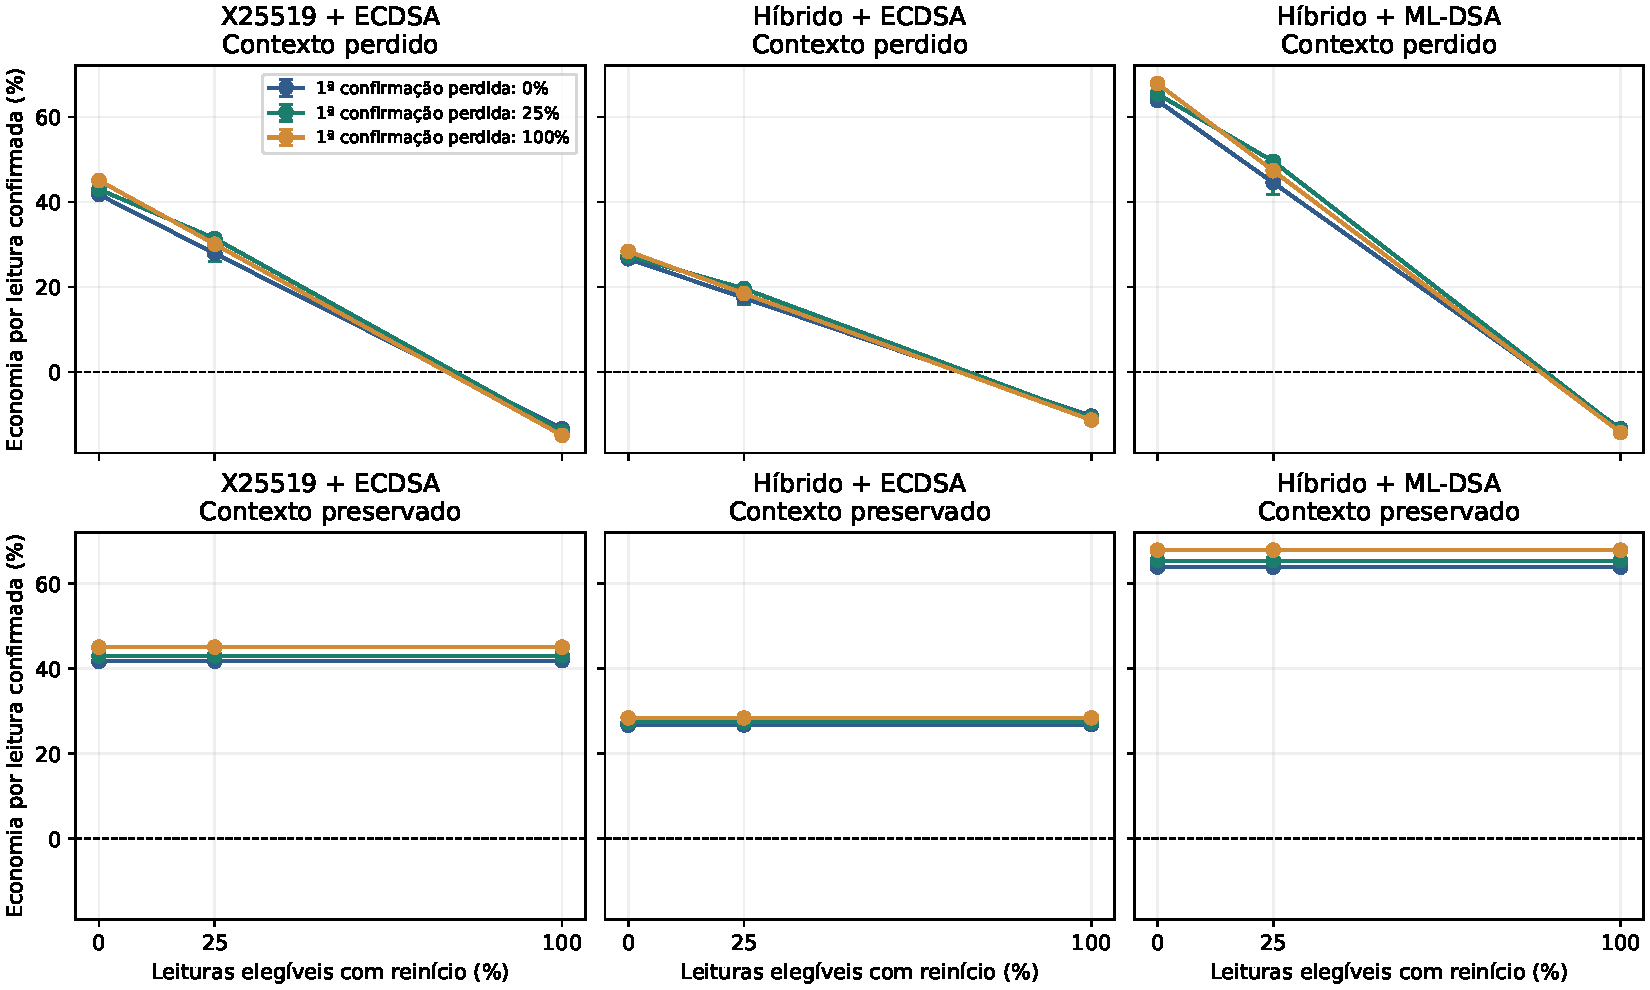
\includegraphics[width=\linewidth]{figuras/continuidade/economia_por_falhas.pdf}
\caption{Economia de bytes IPv4 por leitura confirmada frente ao completo direto, com deduplicação ativa e perda de pacotes configurada em 0\%. Hastes representam intervalos bootstrap exploratórios de dez contrastes por bloco. As linhas ligam as frequências medidas.}
\label{fig:continuidade_economia}
\end{figure}

A Figura~\ref{fig:continuidade_economia} mostra que oferecer retomada não garante economia. No perfil PQC, com reinício e confirmação perdida em 25\%, a economia foi de 49,56\% com chave volátil e 65,43\% com preservação. Em 100\%/100\%, a preservação economizou 67,87\% [67,86; 67,90], enquanto a chave volátil produziu economia negativa de -14,24\% [-14,31; -14,15], isto é, aumento de custo. Nesse cenário, as medianas de bytes por leitura foram 57.489,44 no completo, 65.673,67 no volátil e 18.469,00 no preservado. Os percentuais são contrastes pareados, não razões entre essas medianas.

A inversão também ocorreu no clássico: em 100\%/100\%, o aumento foi de 14,91\% com chave volátil, contra economia de 45,07\% com preservação. No intermediário, os valores foram aumento de 11,31\% e economia de 28,42\%. A diferença absoluta entre políticas cresce com o perfil PQC, mas o problema não é exclusivo dessa configuração.

Uma análise posterior dos 21.960 ClientHello mediu identidades PSK de 640 bytes no clássico, 640--656 no intermediário e 4.240 no PQC. No último, a extensão acrescenta 4.303 bytes à mensagem inicial. Quando o ticket é recusado, esse material acompanha a conexão que executa autenticação completa. A análise mede comprimentos públicos, sem decifrar tickets; diferenças de codificação ECDSA impedem atribuir cada byte a uma única primitiva.

\begin{figure}[!htbp]
\centering
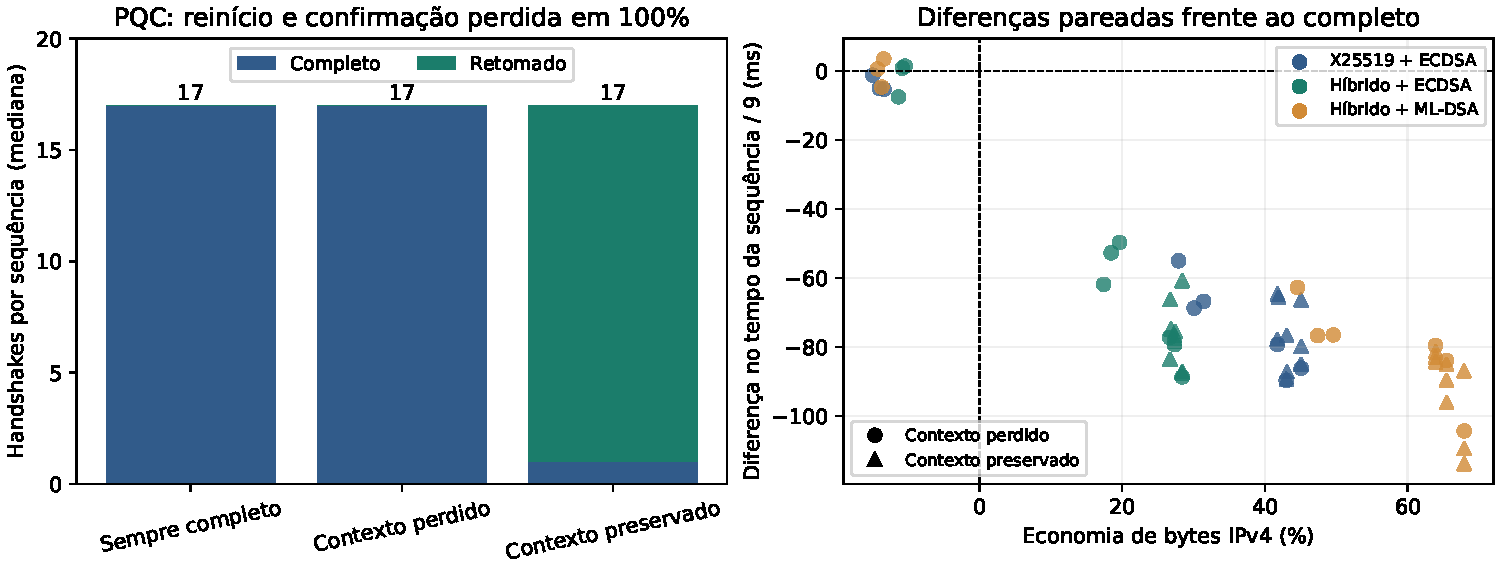
\includegraphics[width=\linewidth]{figuras/continuidade/handshakes_e_tempo.pdf}
\caption{À esquerda, contagens no PQC com falhas lógicas em 100\% das leituras elegíveis. À direita, contrastes temporais e de bytes na matriz principal com deduplicação ativa. O tempo corresponde à sequência até a última confirmação dividida por nove; os pontos são medianas de contrastes por bloco.}
\label{fig:continuidade_contagens}
\end{figure}

Na Figura~\ref{fig:continuidade_contagens}, completo e volátil executam 17 handshakes completos, contra um completo e 16 retomados com preservação. Após a interrupção abrupta, a primeira tentativa não conserva uma sessão substituta utilizável; o ticket antigo permanece inválido quando a chave foi perdida. As contagens de todos os ensaios foram compatíveis com esse mecanismo. Isso explica os custos observados, sem constituir um protocolo novo nem generalizar o comportamento para encerramentos normais ou perdas isoladas de pacotes.

Na fatia PQC de 25\%/25\%, a preservação economizou 65,43\% e 65,45\% sob perdas de 1\% e 5\%. As diferenças pareadas de tempo da sequência por leitura foram -72,09 ms [-91,75; 24,92] e -42,32 ms [-212,56; 160,62]. Como os intervalos incluem zero, não se estabelece superioridade temporal geral sob perda, apesar da economia de bytes.

Todas as 16.200 leituras foram confirmadas em 21.960 tentativas nas matrizes finais. Na principal, cada modo de deduplicação contém 810 ensaios e 7.290 leituras: houve zero efeitos duplicados com supressão e 2.700 no controle. Os 180 ensaios adicionais com supressão também apresentaram zero. As chaves novas e o reconhecimento de leituras cumprem funções distintas; a proteção cobre efeitos gravados na transação com histórico atualizado, sem garantir execução única de atuadores externos ou resistência a rollback conjunto.

Um diagnóstico posterior, separado da matriz, confirmou envio de folha e CA raiz pelo servidor nos três perfis. Isso aumenta o custo completo, especialmente com ML-DSA. Os contrastes valem para essa configuração comum; a magnitude dos percentuais depende da cadeia, e a variante sem transmissão da raiz permanece por avaliar. Não se compara diretamente essa economia com implementações de autenticação ou cadeias diferentes.

A execução principal incorpora blocos completos de sessões distintas, com procedência e hashes registrados. Blocos interrompidos por indisponibilidade de rede ou descarte na captura foram refeitos inteiros, sem selecionar resultados pelo ganho observado. O buffer foi ampliado nos dois últimos blocos e na fase de perdas; todas as capturas incluídas passaram pelo mesmo critério de zero descartes. Dez blocos, um host compartilhado e um sensor delimitam a interpretação temporal e a generalização da avaliação.

\FloatBarrier
